\subsubsection{pair selection}
\label{pair_selection}
It is shown that the channel conditions of users has significant impact to 
the gain in Fig.~\ref{fig_ideal_gain} according to the mathematical model 
of SIC. 
Obviously, the greater difference of channel gain, the more capacity gain 
can be reached theoretically.

In Fig.~\ref{fig_sim_modVSpos}, two user equipments is served by single 
base station and for each point in the figure is a test case of combination
of position.
Users in this simulation can choose its modulation, QPSK or 16QAM, if there
exists an feasible solution of power allocation factor that guarantees the
BER of both users is less than a given threshold.
The figure plots only the highest possible order of modulation user can reach.
Here, the BER threshold is set to be $10^{-2}$.
Fig~\ref{fig_sim_modVSpos} also shows that to maintain a certain level of
QOS in BER, the position of the users is constrained by the far-end user.
This is fine by principle that to prevent error propagation in multi-phase
decoding, the error rate of the data decoded previously (far-end user's data)
has to be controlled.

Moreover, it is verified that the greater difference of distance, the more 
capacity gain can be reached by simulation.
Since the channel gain is a monotonically decreasing function of distance,
greater difference in distance indicates greater difference of channel gain.
For example, assume the far-end user is positioned at a distance of $800$ meter.
Near-end user can only operates at QPSK modulation if it's positioned at
$700$ or $800$, where the channel condition is close to near-end user.
As the near-end user move close to the base station, higher order of modulation
is possible for both users.

\begin{figure}[t]
\begin{center}
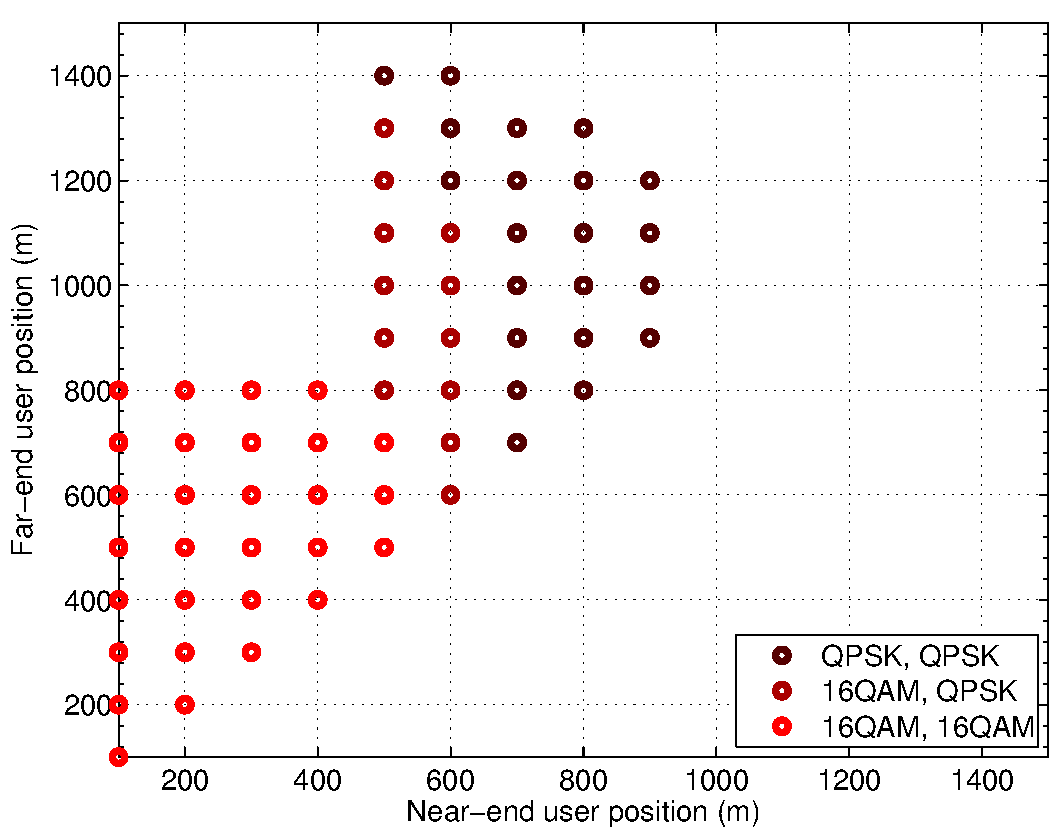
\includegraphics[width=0.95\columnwidth ,angle=0]{figure/positionVSmod.pdf}
\caption{Modulation supported by given BER threshold $10^{-2}$ in two user case}
\label{fig_sim_modVSpos}
\end{center}
\end{figure}

To provide quality service in wireless multiple access network, it's essential
to make proper scheduling between users when the resources is limited. 
To exploit the properties of SIC we've observed in previous simulation, we
further make a experimental scheduling algorithm in a simple scenario.

In Fig.~\ref{fig_sim_topo} shows the topology we use in the simulation.
10 users are randomly scattered in 1400 square meter plane.
Each user has to transmit at least once, and the base station allows at most
2 users to scheduled in a single resource block.
The BER threshold is $10^{-2}$ here.
In short, we have to schedule all users in 5 resource blocks with 2 users in
each with no overlapping. 
By the properties of SIC, we would like to put two user with sufficient difference
in channel gain.

First, we sort all 10 users by the distance in decreasing order, and start 
scheduling form the farthest one, then scan the rest and find the best one
with the highest spectrum efficiency.
Next, remove the pair of users form the scheduling set of users, perform
the same process iteratively.
Finally, we get a schedule and the corresponding power allocation factor $\alpha$
shown in Table~\ref{tb_sim_schedule}.
The alpha listed below each pair is a single point of solution in feasible region.
The simulation shows possible strategy for pair selection in scheduling users
with SIC functionality.

\begin{figure}[t]
\begin{center}
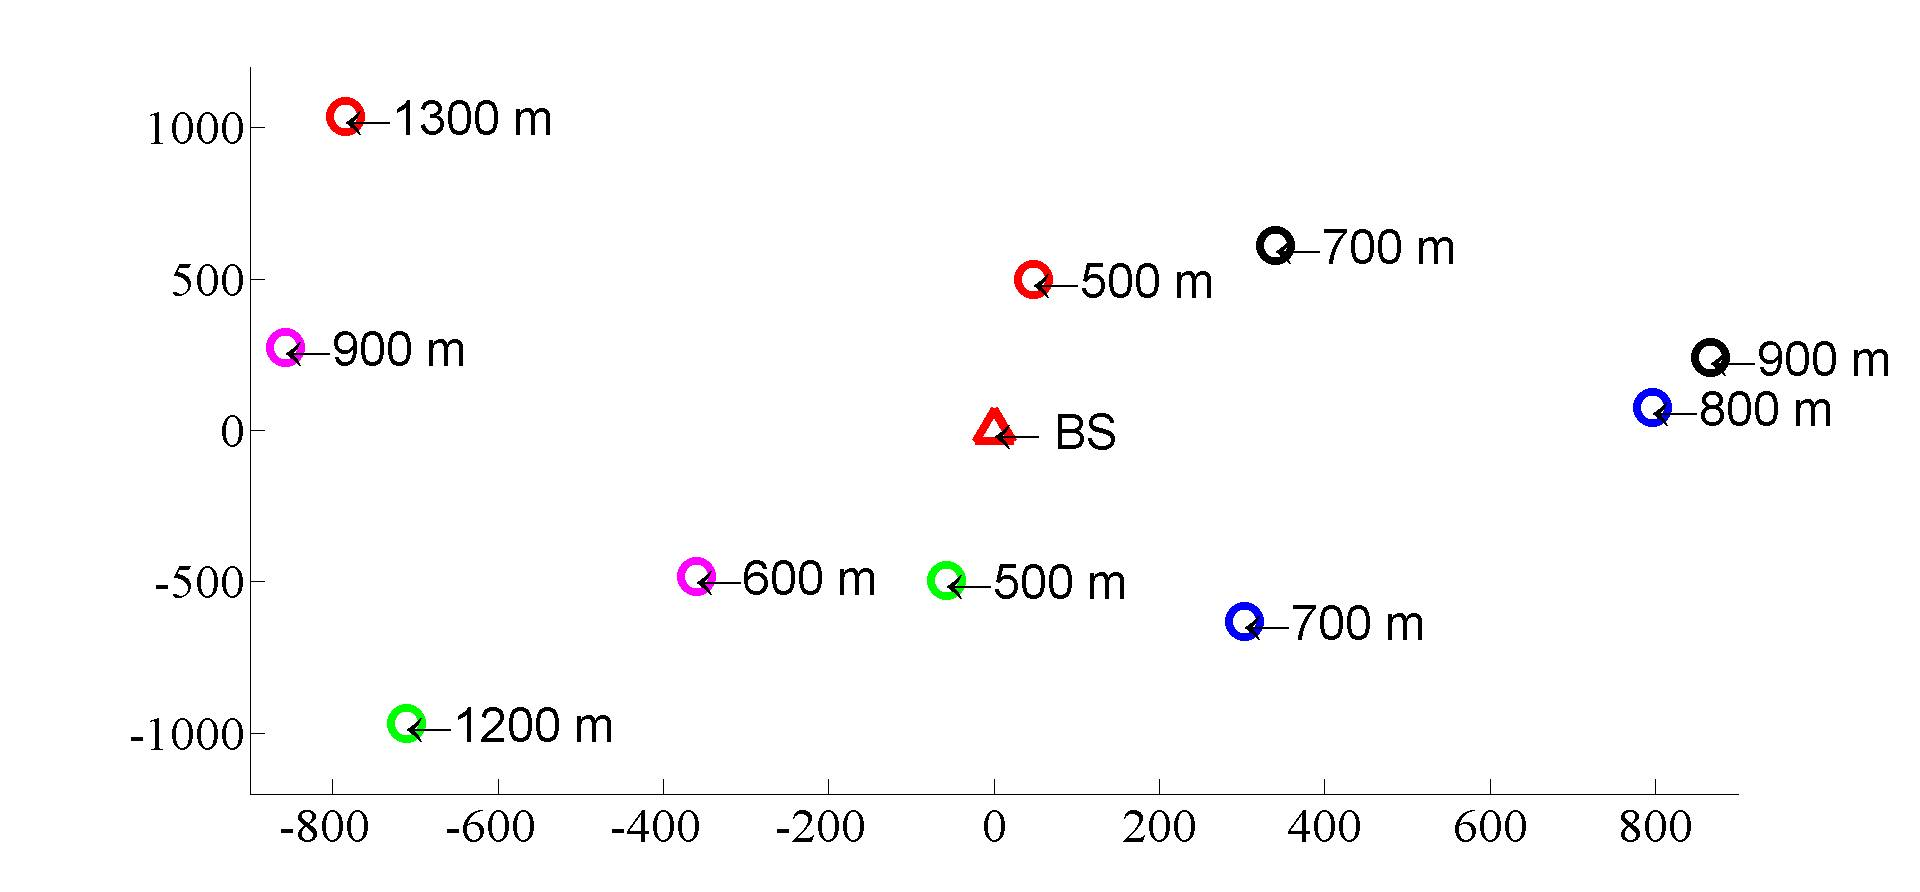
\includegraphics[width=0.95\columnwidth ,angle=0]{figure/topoSimple.jpg}
\caption{Topology of 10 randomly scattered users}
\label{fig_sim_topo}
\end{center}
\end{figure}

\begin{table}[t]
\footnotesize
\caption{Schedule results for each resource block}
    \begin{tabular}{| l | l | l | l | l |}
    \hline
    RB \#1 & RB \#2 & RB \#3 & RB \#4 & RB \#5\\ \hline
    QPSK-1300   &QPSK-700 &QPSK-900    &QPSK-1200  &16QAM-600\\ \hline
    16QAM-500  &QPSK-800 &QPSK-700    &16QAM-500 &QPSK-900\\ \hline \hline
    $\alpha$ value &     &           &     & \\ \hline
    0.1&0.3&0.3&0.075&0.025\\ \hline
    \end{tabular}
\label{tb_sim_schedule}
\end{table}
